\section{Architecture générale de la solution}%
\label{sec.conception.archi}

Pour résoudre le problème de la réhabilitation de la parole aphasique,
nous proposons un système dont l'architecture générale est illustrée dans la Figure~\ref{fig.archi}.
Ce système est composé de deux parties principales :
\begin{enumerate*}[label=(\alph*)]
    \item le sous-système d'\gls{asr} qui permet de transcrire la parole aphasique en texte
    (partie gauche) et
    \item le sous-système de \gls{nmt} qui permet de traduire le texte transcrit en parole saine
    (partie droite).
\end{enumerate*}

\begin{figure}[hbt]
    \begin{center}
        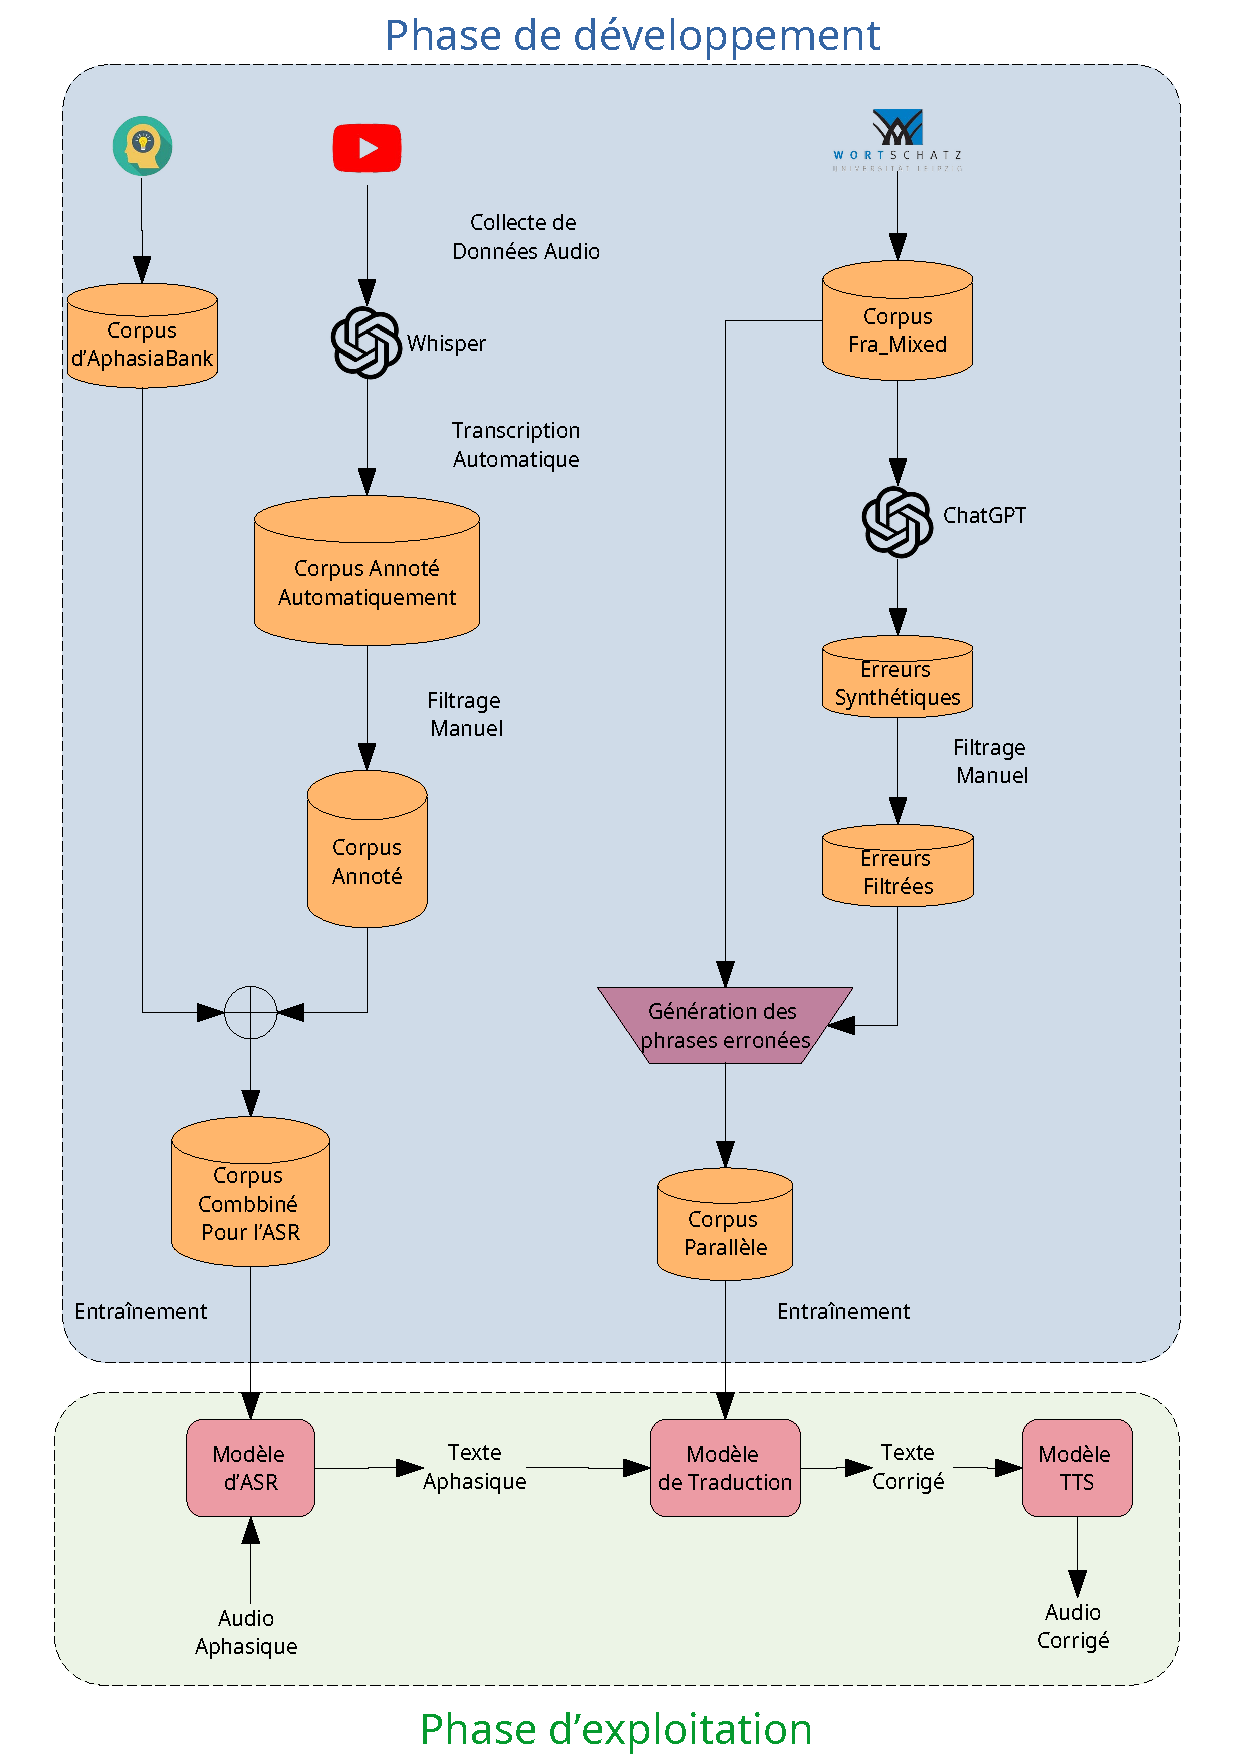
\includegraphics[width=.7\textwidth]{assets/pdf/archutecture.pdf}
    \end{center}
    \caption{Architecture générale de la solution.}
    \label{fig.archi}
\end{figure}

Pour la partie \gls{asr}, nous avons commencé par la collecte de données existantes d'AphasiaBank.
Ces données n'étant pas suffisantes, nous avons collecté des données supplémentaires sur internet.
Ces dernières ont été transcrites automatiquement à l'aide de \foreignlanguage{english}{Whisper}.
Les transcriptions automatiques ont été filtrées manuellement pour corriger les erreurs de transcription.
Le résultat de cette étape est combiné avec les données d'AphasiaBank 
pour former un corpus de données de parole aphasique.
Si ce corpus est de taille suffisante, il peut être utilisé pour entraîner un modèle \gls{asr}.
Cependant, dans notre cas, le corpus est trop petit pour que cela soit possible.

Une fois les deux modèles entraînés,
ils peuvent être enchainés pour former un système ``\foreignlanguage{english}{speech-to-speech}''
(la phase d'exploitation dans la figure \ref{fig.archi}).
Dans la suite de ce chapitre, 
nous reprenons dans le détail les différentes étapes de cette architecture, 
que nous avons abordées brièvement dans cette section.
